\subsection{Input features} \label{inputfeatures}

    \subsubsection{Global features}

        \paragraph{Protein length}
	
  	    Protein length is computed as the number of residues in the protein sequence.
	    It provides complementary information that convolutional layers cannot capture.
 	    Indeed, fully-connected neural networks have the ability to handle arbitrary-sized
	    features maps at the cost of not knowing the dimensionality of their inputs.
	    Injecting protein length as a supplementary global feature may help the model
	    to infer the maximum distance in long-range contacts.

	\paragraph{Effective number of sequences}

	    The number of effective sequences is equal, w.r.t. to a given threshold,
	    to the number of non-redundant sequences in the set of homologous sequences.
	    It provides a bound on the potential performance of the DCA methods involved
	    in the pipeline.

        \paragraph{Predictors standard deviation}

    \subsubsection{1-dimensional features}

        \paragraph{One-hot encoded sequence}

            Given an amino acid sequence $\{s_1, s_2, \ldots,
            s_L\}$ of size L, its one-hot encoded version
            is a matrix $X \in \{0, 1\}^{L \times 21}$
            where $x_{ia}$ is one if $s_i = a$.

        \paragraph{Solvent accessibility}

            \todo{}

            \begin{figure}[H]
                \begin{center}
                    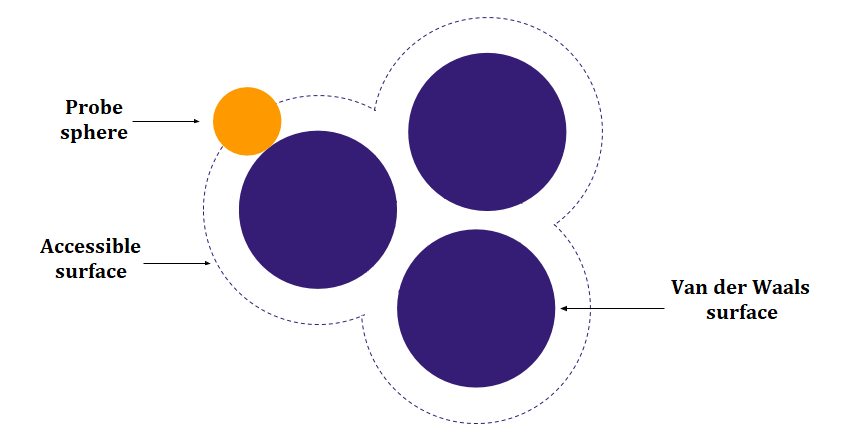
\includegraphics[height=5cm, keepaspectratio]{imgs/accessibility.png}
                    \caption{Accessible surface, obtained by "rolling" a probe sphere (a molecule
                        of solvent, colored in orange) on the Van der Waals surface of a biomolecule
                        (colored in blue).}
                    \label{architecture}
                \end{center}
            \end{figure}


        \paragraph{Predicted Secondary Structure Prediction}

        \paragraph{Amino acid frequencies}

            Amino acid frequencies are position-specific features that can be efficiently computed.
            Let $S \in \{0, \ldots, \naatypes\}^{M \times L}$ be a 
            MSA matrix containing $M$ sequences aligned to a target
            sequence of length $L$. Then amino acid frequencies can be arranged
            in a matrix $F \in \mathbb{R}^{L \times \naatypes}$
            where element $F_{ia}$ is computed as follows:

            \begin{equation}
                F_{ia} = \frac{1}{M} \sum\limits_{k=1}^M \delta(S_{ki}, a)
            \end{equation}

        \paragraph{Position-Specific Scoring Matrix}

            \todo{PSI-PRED: \cite{jones1999protein}}

        \paragraph{Atchley factors}

            \todo{Atchley: \cite{Atchley2005}}

        \paragraph{Self-information}

            In information theory, self-information is the amount of information, in bits,
            obtained by observing a random variable. In particular, let $x_{ij} \in \{0, 1\}$ be
            a binary variable indicating the presence of an amino acid of type $j$ at site $i$.
            The self-information suggested by Michel et al~\cite{Michel383133} can be formalized
            with the following equation:

            \begin{equation}
                I_{ij} = \log_2 (p_{ij} / \langle p_i \rangle)
            \end{equation}

            where $p_{ij}$ is the probability of observing amino acid $j$ at site $i$ among all residues
            of given MSA, and $\langle p_j \rangle$ is the frequency of amino acid $j$
            in the Uniref50 dataset.

        \paragraph{Partial entropies}

            \cite{Michel383133}

            \begin{equation}
                S_i = p_i \log_2 (p_i / \langle p_i \rangle)
            \end{equation}

    \subsubsection{2-dimensional features}

        \paragraph{Mutual Information and Normalized Mutual Information}

            Following the formalism described in \cite{Michel383133}, MI is described as:

            \begin{equation}
                MI(x, y) = \sum\limits_{x, y} P(x, y) \log \Big( \frac{P(x, y)}{P(x) P(y)} \Big)
            \end{equation}

            \begin{equation}
                NMI(x, y) = \frac{MI(x, y)}{\sqrt{S(x) S(y)}}
            \end{equation}

            APC is applied to both MI and NMI.

        \paragraph{Cross-entropy}

            Cross-entropy is computed in \cite{Michel383133} using the following formula:
            
            \begin{equation}
                H(x, y) = S(x) + S(y) - MI(x, y)
            \end{equation}

        \paragraph{Contact potential}

        \paragraph{Predictions from DCA and PSICOV}

        \paragraph{Covariance}

    \subsection{Features, by method}

        \begin{figure}[H]
            \begin{center}
                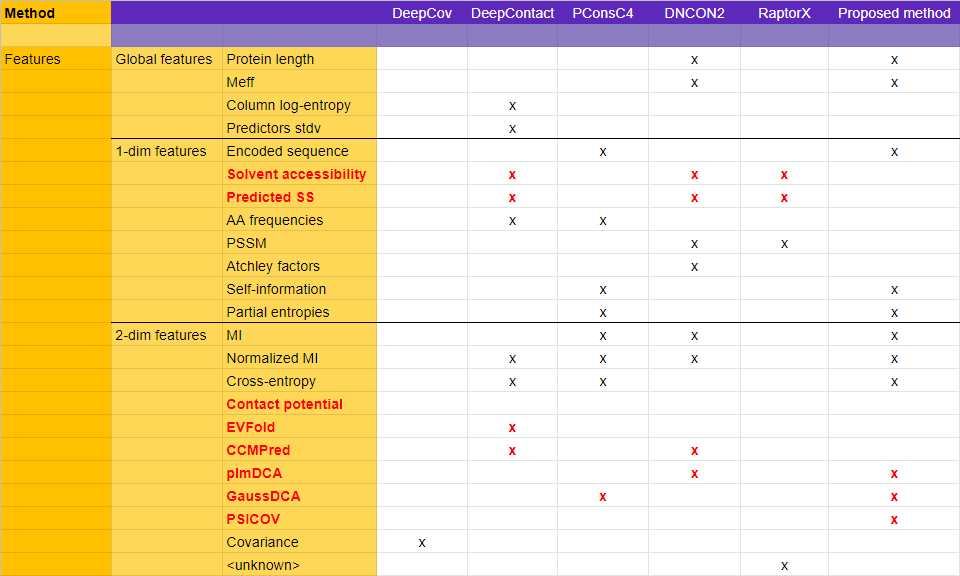
\includegraphics[width=\textwidth, keepaspectratio]{imgs/features.png}
                \caption{Features used in state-of-the-art deep learning approaches.
                Feature extraction methods that rely on external tools (excluding
                MSA tools) are highlighted in red.}
                \label{features}
            \end{center}
        \end{figure}